\chapter{Implementation}

The following chapter describes how the protoype has been implemented and the materials needed to build the prototype. 

\subsection{Hardware}

The prototype consists of an Arduino Mega 2560\citep{Arduino}, which is connected to a circuit board with an inertial measurement unit(IMU). 
The IMU uses the MPU 9150 sensor with 9 degrees of freedom\citep{MPU}. It has a tri-axis gyroscope, magnetometer, and accelorometer.

\subsection{Schematic} 

The following figure \ref{schematic} shows how the Arduino is connected to the circuit board with the IMU. The black switch at the top of the circuit board
represents the three connections, which is put on the thumb, index and middle finger. These are velcro based, with copper tape on them, to create the connection when pressed together. 

\begin{minipage}{\linewidth}% to keep image and caption on one page
\makebox[\linewidth]{%        to center the image
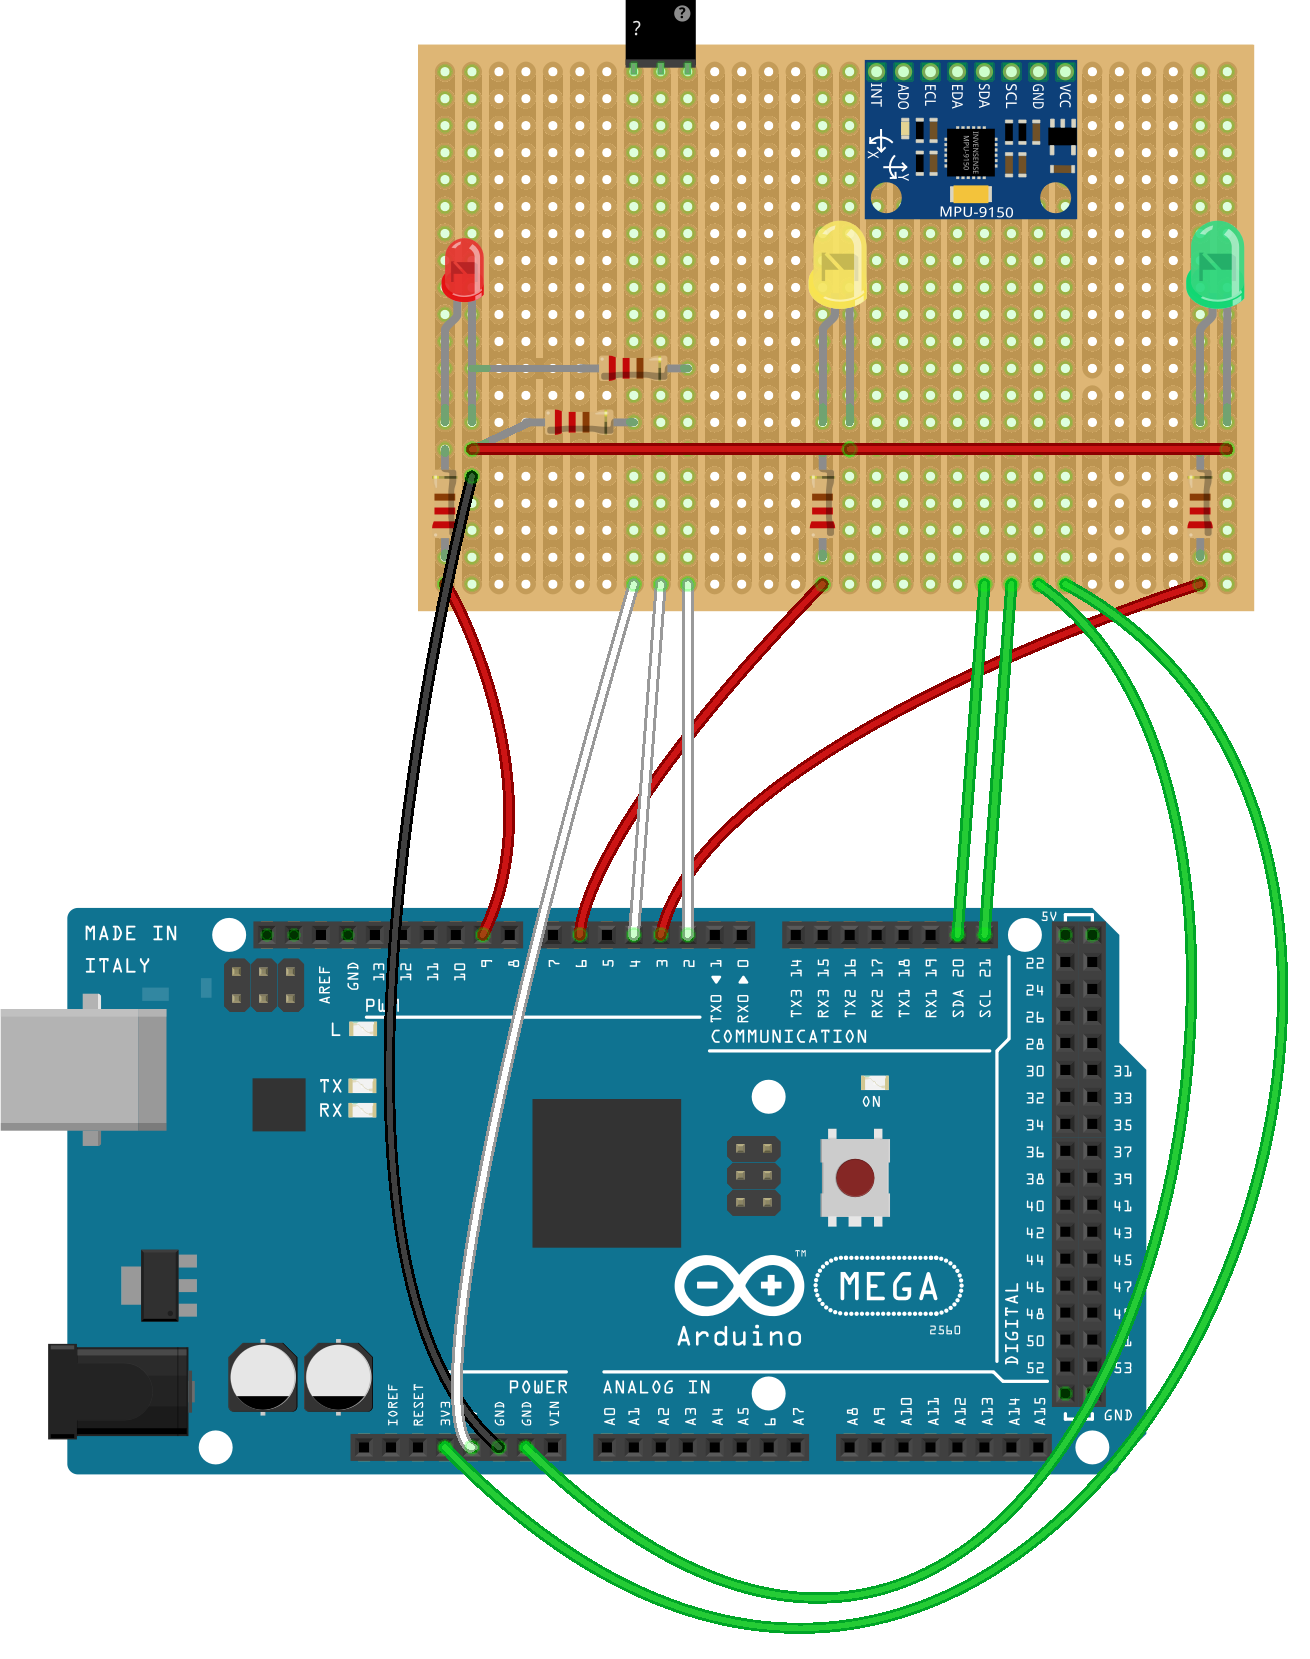
\includegraphics[keepaspectratio=true,scale=1.2]{Imu_Glove_Schematic}}
\captionof{figure}{Prototype Schematic}\label{schematic}
\end{minipage}\\

The circuit board consists of three LEDs, a yellow, green and red. They light up at different points, which is explained in the next section of this chapter.
The LEDs are connected to resistors of 220 ohm which is wired to the arduino as seen in the schematic. The LEDs has to be connected to a pull-down resistor\citep{Pull_down_res},
which makes sure, that the Arduino does not 'float' between two different values. A pull-down resistor ensures, that the value is zero, when no active device is connected.
The following figure \ref{Pull_down_res} shows what a circuit with a pull-down resistor might look like. 

%Five 220 ohm resistors (Two Pull-down resistor), three LEDs red, yellow, green. Copper tape. RedS Tape and velcro. 

\begin{minipage}{\linewidth}% to keep image and caption on one page
\makebox[\linewidth]{%        to center the image
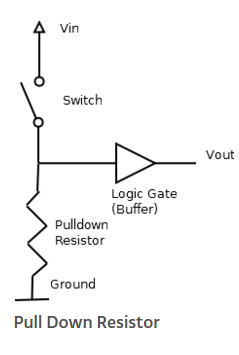
\includegraphics[keepaspectratio=true,scale=0.7]{Pull_down_resistor}}
\captionof{figure}{Schematic of Pull-down resistor\citep{Pull_down_res}}\label{pull_down}
\end{minipage}\\

\subsection{Software}

The Arduino language is based on C/C++, and whenever a sketch is compiled, it is sent to a C/C++ compiler \citep{Arduino_FAQ}.

%Arduino
%PD